\documentclass{standalone}
\usepackage{tikz}
\usetikzlibrary{patterns, positioning}

\begin{document}
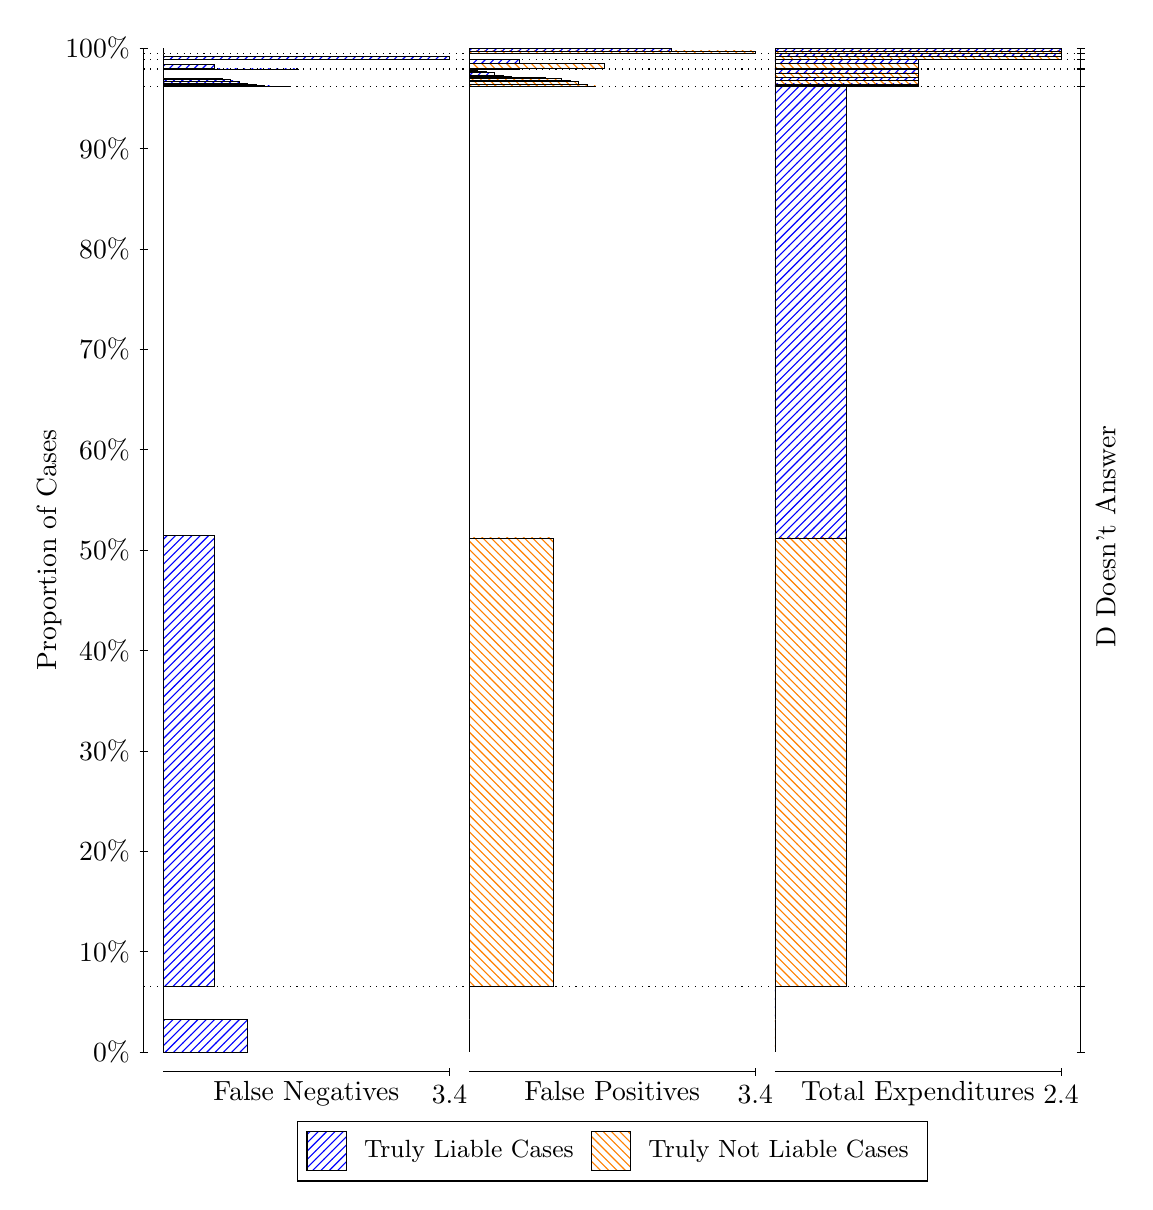
\begin{tikzpicture}
\draw[black, very thin] (1.5,1.75) -- (1.5,14.5);
\node[rotate=90, anchor=center] at (0.3, 8.125) {Proportion of Cases};
\draw[black, very thin] (1.45,1.75) -- (1.55,1.75);
\node[anchor=east] at (1.45, 1.75) {0\%};
\draw[black, very thin] (1.45,3.025) -- (1.55,3.025);
\node[anchor=east] at (1.45, 3.025) {10\%};
\draw[black, very thin] (1.45,4.3) -- (1.55,4.3);
\node[anchor=east] at (1.45, 4.3) {20\%};
\draw[black, very thin] (1.45,5.575) -- (1.55,5.575);
\node[anchor=east] at (1.45, 5.575) {30\%};
\draw[black, very thin] (1.45,6.85) -- (1.55,6.85);
\node[anchor=east] at (1.45, 6.85) {40\%};
\draw[black, very thin] (1.45,8.125) -- (1.55,8.125);
\node[anchor=east] at (1.45, 8.125) {50\%};
\draw[black, very thin] (1.45,9.4) -- (1.55,9.4);
\node[anchor=east] at (1.45, 9.4) {60\%};
\draw[black, very thin] (1.45,10.675) -- (1.55,10.675);
\node[anchor=east] at (1.45, 10.675) {70\%};
\draw[black, very thin] (1.45,11.95) -- (1.55,11.95);
\node[anchor=east] at (1.45, 11.95) {80\%};
\draw[black, very thin] (1.45,13.225) -- (1.55,13.225);
\node[anchor=east] at (1.45, 13.225) {90\%};
\draw[black, very thin] (1.45,14.5) -- (1.55,14.5);
\node[anchor=east] at (1.45, 14.5) {100\%};

\draw[black, very thin] (13.4,1.75) -- (13.4,14.5);
\draw[black, very thin] (13.35,1.75) -- (13.45,1.75);
\node[anchor=west] at (13.35, 1.75) {};
\draw[black, very thin] (13.35,2.5802) -- (13.45,2.5802);
\node[anchor=west] at (13.35, 2.5802) {};
\draw[black, very thin] (13.35,14.01) -- (13.45,14.01);
\node[anchor=west] at (13.35, 14.01) {};
\draw[black, very thin] (13.35,14.231) -- (13.45,14.231);
\node[anchor=west] at (13.35, 14.231) {};
\draw[black, very thin] (13.35,14.24) -- (13.45,14.24);
\node[anchor=west] at (13.35, 14.24) {};
\draw[black, very thin] (13.35,14.358) -- (13.45,14.358);
\node[anchor=west] at (13.35, 14.358) {};
\draw[black, very thin] (13.35,14.43) -- (13.45,14.43);
\node[anchor=west] at (13.35, 14.43) {};
\draw[black, very thin] (13.35,14.5) -- (13.45,14.5);
\node[anchor=west] at (13.35, 14.5) {};

\draw[black, very thin, pattern color=blue, pattern=north east lines] (1.75,1.75) rectangle (2.8186,2.1651);
\draw[black, very thin, pattern color=orange, pattern=north west lines] (1.75,2.1651) rectangle (1.75,2.5802);
\draw[black, very thin, pattern color=blue, pattern=north east lines] (1.75,2.5802) rectangle (2.3912,8.3115);
\draw[black, very thin, pattern color=orange, pattern=north west lines] (1.75,8.3115) rectangle (1.75,14.01);
\draw[black, very thin, pattern color=blue, pattern=north east lines] (1.75,14.01) rectangle (3.3529,14.012);
\draw[black, very thin, pattern color=blue, pattern=north east lines] (1.75,14.012) rectangle (3.2461,14.014);
\draw[black, very thin, pattern color=blue, pattern=north east lines] (1.75,14.014) rectangle (3.1392,14.02);
\draw[black, very thin, pattern color=blue, pattern=north east lines] (1.75,14.02) rectangle (3.0324,14.025);
\draw[black, very thin, pattern color=blue, pattern=north east lines] (1.75,14.025) rectangle (2.9255,14.041);
\draw[black, very thin, pattern color=blue, pattern=north east lines] (1.75,14.041) rectangle (2.8186,14.055);
\draw[black, very thin, pattern color=blue, pattern=north east lines] (1.75,14.055) rectangle (2.7118,14.084);
\draw[black, very thin, pattern color=blue, pattern=north east lines] (1.75,14.084) rectangle (2.6049,14.103);
\draw[black, very thin, pattern color=blue, pattern=north east lines] (1.75,14.103) rectangle (2.498,14.112);
\draw[black, very thin, pattern color=orange, pattern=north west lines] (1.75,14.112) rectangle (1.75,14.231);
\draw[black, very thin, pattern color=blue, pattern=north east lines] (1.75,14.231) rectangle (3.4598,14.235);
\draw[black, very thin, pattern color=orange, pattern=north west lines] (1.75,14.235) rectangle (1.75,14.24);
\draw[black, very thin, pattern color=blue, pattern=north east lines] (1.75,14.24) rectangle (2.3912,14.295);
\draw[black, very thin, pattern color=orange, pattern=north west lines] (1.75,14.295) rectangle (1.75,14.358);
\draw[black, very thin, pattern color=blue, pattern=north east lines] (1.75,14.358) rectangle (5.3833,14.389);
\draw[black, very thin, pattern color=orange, pattern=north west lines] (1.75,14.389) rectangle (1.75,14.43);
\draw[black, very thin, pattern color=orange, pattern=north west lines] (1.75,14.43) rectangle (1.75,14.464);
\draw[black, very thin, pattern color=blue, pattern=north east lines] (1.75,14.464) rectangle (1.75,14.5);
\draw[black, very thin, pattern color=orange, pattern=north west lines] (5.6333,1.75) rectangle (5.6333,2.1651);
\draw[black, very thin, pattern color=blue, pattern=north east lines] (5.6333,2.1651) rectangle (5.6333,2.5802);
\draw[black, very thin, pattern color=orange, pattern=north west lines] (5.6333,2.5802) rectangle (6.702,8.2786);
\draw[black, very thin, pattern color=blue, pattern=north east lines] (5.6333,8.2786) rectangle (5.6333,14.01);
\draw[black, very thin, pattern color=orange, pattern=north west lines] (5.6333,14.01) rectangle (7.2363,14.02);
\draw[black, very thin, pattern color=orange, pattern=north west lines] (5.6333,14.02) rectangle (7.1294,14.042);
\draw[black, very thin, pattern color=orange, pattern=north west lines] (5.6333,14.042) rectangle (7.0225,14.076);
\draw[black, very thin, pattern color=orange, pattern=north west lines] (5.6333,14.076) rectangle (6.9157,14.092);
\draw[black, very thin, pattern color=orange, pattern=north west lines] (5.6333,14.092) rectangle (6.8088,14.111);
\draw[black, very thin, pattern color=orange, pattern=north west lines] (5.6333,14.111) rectangle (6.702,14.117);
\draw[black, very thin, pattern color=orange, pattern=north west lines] (5.6333,14.117) rectangle (6.5951,14.124);
\draw[black, very thin, pattern color=orange, pattern=north west lines] (5.6333,14.124) rectangle (6.4882,14.127);
\draw[black, very thin, pattern color=orange, pattern=north west lines] (5.6333,14.127) rectangle (6.3814,14.129);
\draw[black, very thin, pattern color=blue, pattern=north east lines] (5.6333,14.129) rectangle (6.1676,14.138);
\draw[black, very thin, pattern color=blue, pattern=north east lines] (5.6333,14.138) rectangle (6.0608,14.157);
\draw[black, very thin, pattern color=blue, pattern=north east lines] (5.6333,14.157) rectangle (5.9539,14.187);
\draw[black, very thin, pattern color=blue, pattern=north east lines] (5.6333,14.187) rectangle (5.8471,14.2);
\draw[black, very thin, pattern color=blue, pattern=north east lines] (5.6333,14.2) rectangle (5.7402,14.216);
\draw[black, very thin, pattern color=blue, pattern=north east lines] (5.6333,14.216) rectangle (5.6333,14.231);
\draw[black, very thin, pattern color=orange, pattern=north west lines] (5.6333,14.231) rectangle (6.2745,14.236);
\draw[black, very thin, pattern color=blue, pattern=north east lines] (5.6333,14.236) rectangle (5.6333,14.24);
\draw[black, very thin, pattern color=orange, pattern=north west lines] (5.6333,14.24) rectangle (7.3431,14.303);
\draw[black, very thin, pattern color=blue, pattern=north east lines] (5.6333,14.303) rectangle (6.2745,14.358);
\draw[black, very thin, pattern color=orange, pattern=north west lines] (5.6333,14.358) rectangle (5.6333,14.399);
\draw[black, very thin, pattern color=blue, pattern=north east lines] (5.6333,14.399) rectangle (5.6333,14.43);
\draw[black, very thin, pattern color=orange, pattern=north west lines] (5.6333,14.43) rectangle (9.2667,14.464);
\draw[black, very thin, pattern color=blue, pattern=north east lines] (5.6333,14.464) rectangle (8.198,14.5);
\draw[black, very thin, pattern color=orange, pattern=north west lines] (9.5167,1.75) rectangle (9.5167,2.1651);
\draw[black, very thin, pattern color=blue, pattern=north east lines] (9.5167,2.1651) rectangle (9.5167,2.5802);
\draw[black, very thin, pattern color=orange, pattern=north west lines] (9.5167,2.5802) rectangle (10.425,8.2786);
\draw[black, very thin, pattern color=blue, pattern=north east lines] (9.5167,8.2786) rectangle (10.425,14.01);
\draw[black, very thin, pattern color=orange, pattern=north west lines] (9.5167,14.01) rectangle (11.333,14.028);
\draw[black, very thin, pattern color=blue, pattern=north east lines] (9.5167,14.028) rectangle (11.333,14.044);
\draw[black, very thin, pattern color=orange, pattern=north west lines] (9.5167,14.044) rectangle (11.333,14.088);
\draw[black, very thin, pattern color=blue, pattern=north east lines] (9.5167,14.088) rectangle (11.333,14.127);
\draw[black, very thin, pattern color=orange, pattern=north west lines] (9.5167,14.127) rectangle (11.333,14.183);
\draw[black, very thin, pattern color=blue, pattern=north east lines] (9.5167,14.183) rectangle (11.333,14.231);
\draw[black, very thin, pattern color=orange, pattern=north west lines] (9.5167,14.231) rectangle (11.333,14.236);
\draw[black, very thin, pattern color=blue, pattern=north east lines] (9.5167,14.236) rectangle (11.333,14.24);
\draw[black, very thin, pattern color=orange, pattern=north west lines] (9.5167,14.24) rectangle (11.333,14.303);
\draw[black, very thin, pattern color=blue, pattern=north east lines] (9.5167,14.303) rectangle (11.333,14.358);
\draw[black, very thin, pattern color=orange, pattern=north west lines] (9.5167,14.358) rectangle (13.15,14.399);
\draw[black, very thin, pattern color=blue, pattern=north east lines] (9.5167,14.399) rectangle (13.15,14.43);
\draw[black, very thin, pattern color=orange, pattern=north west lines] (9.5167,14.43) rectangle (13.15,14.464);
\draw[black, very thin, pattern color=blue, pattern=north east lines] (9.5167,14.464) rectangle (13.15,14.5);
\draw[black, dotted] (1.5,2.5802) -- (13.4,2.5802);
\draw[black, dotted] (1.5,14.01) -- (13.4,14.01);
\draw[black, dotted] (1.5,14.231) -- (13.4,14.231);
\draw[black, dotted] (1.5,14.24) -- (13.4,14.24);
\draw[black, dotted] (1.5,14.358) -- (13.4,14.358);
\draw[black, dotted] (1.5,14.43) -- (13.4,14.43);
\draw[black, very thin] (1.75,1.5) -- (5.3833,1.5);
\node[anchor=north] at (3.5667, 1.5) {False Negatives};
\draw[black, very thin] (5.3833,1.45) -- (5.3833,1.55);
\node[anchor=north] at (5.3833, 1.45) {3.4};

\draw[black, very thin] (5.6333,1.5) -- (9.2667,1.5);
\node[anchor=north] at (7.45, 1.5) {False Positives};
\draw[black, very thin] (9.2667,1.45) -- (9.2667,1.55);
\node[anchor=north] at (9.2667, 1.45) {3.4};

\draw[black, very thin] (9.5167,1.5) -- (13.15,1.5);
\node[anchor=north] at (11.333, 1.5) {Total Expenditures};
\draw[black, very thin] (13.15,1.45) -- (13.15,1.55);
\node[anchor=north] at (13.15, 1.45) {2.4};


\node[black, centered, rotate=90] at (13.72, 8.295) {D Doesn't Answer};






\draw (7.449999999999999,1.5) node[draw=none] (baseCoordinate) {};
\begin{scope}[align=center]
        \matrix[scale=0.5, draw=black, below=0.5cm of baseCoordinate, nodes={draw}, column sep=0.1cm]{
            \node[rectangle, draw, minimum width=0.5cm, minimum height=0.5cm, pattern=north east lines, pattern color=blue] {}; &
            \node[draw=none, font=\small] (B) {Truly Liable Cases}; &
            \node[rectangle, draw, minimum width=0.5cm, minimum height=0.5cm, pattern=north west lines, pattern color=orange] {}; &
            \node[draw=none, font=\small] (B) {Truly Not Liable Cases}; \\
            };
\end{scope}

\end{tikzpicture}
\end{document}